\documentclass[runningheads]{llncs}
\usepackage[utf8]{inputenc}
\usepackage{lmodern}
\usepackage{graphicx}
\usepackage{amsmath}
\usepackage{amssymb}
\usepackage{booktabs}
\usepackage{hyperref}
\usepackage{multirow}
\usepackage{array}
\hypersetup{hidelinks}
\begin{document}
\title{Activaciones Racionales Condicionadas por Contexto: Cuándo Ayuda Adaptar la No Linealidad}
\author{Agustín Hugo Astie Forconesi \and Juan Pablo Gerino \and Joaquin Imanol Ortega \and Miguel Méndez Garabetti}
\institute{Laboratorio de Investigación en Ciencia y Tecnología,\\ Universidad del Aconcagua, Mendoza, Argentina.\\
\email{agustinastie3@gmail.com, juanpigerino@gmail.com}\\
\email{joaquinimanolortega@gmail.com, mmendez@uda.edu.ar}}
\titlerunning{Activaciones Racionales Condicionadas por Contexto}
\authorrunning{A. Astie et al.}
\maketitle
\pagestyle{empty}
\thispagestyle{empty}

\begin{abstract}
Presentamos la Activación Racional Condicionada por Contexto (CCA), una familia de no linealidades cuyos coeficientes se generan para cada muestra a partir de un resumen global, sin utilizar la etiqueta ni la identidad del dominio durante la inferencia. Su variante confirmatoria, CCA-Hinge, combina una base SiLU, una corrección racional estable y una bisagra suave condicionada; CCA-Lite reduce el generador para priorizar eficiencia. Comparamos directamente ambas variantes con SiLU, una activación racional estática, Dynamic ReLU-B y Meta-ACON. En una evaluación confirmatoria de diez semillas, con presupuestos igualados de parámetros y FLOPs, CCA-Hinge alcanza $88.68\%$ en MNIST+SVHN+USPS y supera a Dynamic ReLU-B por $0.62$ puntos (IC95\% $[0.21,1.11]$, $p_{\mathrm{Holm}}=0.023$); en clasificación de texto queda estadísticamente empatada con las activaciones adaptativas. Una matriz adicional en visión, lenguaje, audio, razonamiento y generación muestra ventajas concentradas en tareas genuinamente multirrégimen, incluido un caso nulo real de sentimiento. Los resultados delimitan la contribución: adaptar la curva resulta útil cuando el contexto cambia la transformación requerida, pero no ofrece una ventaja universal.
\keywords{Aprendizaje profundo \and activaciones adaptativas \and hiperredes \and aprendizaje condicionado \and cambio de dominio.}
\end{abstract}

\section{Introducción}
Una función de activación estática aplica la misma transformación a toda muestra. Esta invariancia es conveniente, pero puede convertirse en un cuello de botella cuando un único modelo debe resolver regímenes incompatibles. Por ejemplo, una representación útil para una imagen normal puede requerir una respuesta distinta después de invertir sus intensidades, o una misma secuencia simbólica puede obedecer diferentes claves de sustitución. El problema no consiste solamente en reconocer el régimen, sino en modificar el cómputo que corresponde a ese régimen.

Proponemos las \textit{Activaciones Racionales Condicionadas por Contexto} (CCA), que generan por muestra los parámetros de una curva estable. La pregunta de investigación es: \emph{¿puede una no linealidad condicionada superar activaciones estáticas y dinámicas bajo el mismo presupuesto, cuando el contexto debe inferirse sin identidad de dominio?} Para responderla separamos dos niveles de evidencia: una comparación confirmatoria con parámetros y FLOPs igualados, y una matriz amplia que mantiene el mismo backbone para todos los métodos.

Las contribuciones son:
\begin{itemize}
\item una activación racional condicionada con inicialización Exact-SiLU y una extensión CCA-Hinge que añade una base de quiebre suave sin perder esa inicialización;
\item una comparación directa contra Dynamic ReLU-B, Meta-ACON y racionales estáticas, con diez semillas emparejadas, IC95\%, pruebas exactas, corrección de Holm y tamaños de efecto;
\item una aplicación real multirrégimen sobre MNIST, SVHN y USPS, donde el contexto se infiere de las preactivaciones y nunca contiene la identidad del dataset;
\item una evaluación reproducible en doce escenarios de texto, imágenes, audio, razonamiento y generación, junto con controles de régimen único y de contexto incorrecto.
\end{itemize}

\section{Trabajo relacionado}
\textbf{Activaciones aprendibles.} Las unidades racionales aproximan funciones suaves con menor profundidad teórica que redes ReLU y permiten aprender numeradores y denominadores \cite{boulle2020rational}. Sin embargo, una activación racional estática aprende una sola curva para todo el conjunto. Dynamic ReLU genera desde un resumen global dos ramas lineales y toma su máximo; su variante B comparte parámetros espacialmente y los adapta por canal \cite{chen2020dynamic}. ACON interpreta la activación como una transición suave entre dos ramas, mientras Meta-ACON predice desde el contexto el factor que controla esa transición \cite{ma2021activate}. En contraste, CCA condiciona simultáneamente un ajuste afín y una corrección racional acotada; CCA-Hinge añade una base tipo Maxout suavizada. Nuestra comparación implementa estas formulaciones mediante una interfaz común y entrega exactamente el mismo contexto a todos los métodos adaptativos.

\textbf{Cómputo condicionado.} Las hiperredes generan parámetros de otra red \cite{ha2017hypernetworks}; FiLM modula características mediante escalas y sesgos \cite{perez2018film}; y CondConv combina núcleos convolucionales dependientes de la muestra \cite{yang2019condconv}. Estas técnicas condicionan pesos o representaciones. CCA aplica el mismo principio a la forma de la no linealidad. El control B0H separa ambos mecanismos: recibe el mismo contexto que CCA, pero lo suma a la representación en lugar de utilizarlo para deformar la curva.

\section{Activación propuesta}
Sea $x$ una preactivación y $c$ un contexto. Un generador pequeño $G(c)$ produce parámetros por grupos de canales. Primero se aplica
\begin{equation}
u=w(c)x+d(c).
\label{eq:affine}
\end{equation}
CCA-Lite calcula
\begin{equation}
A_{\mathrm{lite}}(x,c)=u\sigma(u)+
\alpha\frac{a_0(c)+a_1(c)u+a_2(c)u^2}{1+\left(b_0(c)+b_1(c)u\right)^2}.
\label{eq:cca}
\end{equation}
El denominador es al menos uno y evita polos. El parámetro $\alpha$ se aprende por grupo. CCA-Lite usa 16 grupos y un generador oculto de ancho 16; la versión completa usa 64/64.

CCA-Hinge amplía la base funcional:
\begin{equation}
A_{\mathrm{hinge}}(x,c)=A_{\mathrm{lite}}(x,c)+
\lambda(c)\sqrt{(u-t(c))^2+\epsilon},\qquad \epsilon=10^{-4}.
\label{eq:hinge}
\end{equation}
La amplitud $\lambda(c)$ y el umbral $t(c)$ dependen del contexto. La bisagra suave representa cambios de pendiente que una racional de grado bajo puede requerir más coeficientes para aproximar. En todas las variantes, la última proyección de $G$ se inicializa en cero, $w=1$, $d=0$, los coeficientes racionales y $\lambda$ valen cero, y la red comienza exactamente como SiLU \cite{silu}. Esta condición permite atribuir cualquier desviación posterior al aprendizaje.

La configuración Hinge se eligió únicamente con semillas de desarrollo 2001--2003 y validación separada. Se fijaron 16 grupos y ancho 16 antes de la confirmación sobre semillas nuevas 3001--3010. Ningún resultado de prueba intervino en la selección.

\section{Protocolo experimental}

\subsection{Baselines, presupuesto y estadística}
Comparamos SiLU, SiLU ensanchada, Rational estática, Dynamic ReLU-B con dos ramas, Meta-ACON, CCA-Lite y CCA-Hinge. Todas usan una interfaz común y reciben el mismo contexto cuando son adaptativas. En la comparación confirmatoria se toma CCA-Hinge con el backbone original como presupuesto; una búsqueda discreta ajusta solo el ancho del backbone, los grupos y el generador para quedar dentro de $105\%$ de sus parámetros y $110\%$ de sus FLOPs analíticos. La selección usa exclusivamente costo, nunca exactitud de prueba. La matriz amplia conserva el mismo backbone; sus diferencias de parámetros se publican con los resultados crudos.

Las semillas son emparejadas entre métodos. Las tareas confirmatorias y de clasificación usan diez semillas; la generación por caracteres y la generación de imágenes usan tres por su mayor costo. Reportamos media, desviación estándar e IC95\% percentil con 10\,000 remuestras. Las diferencias de CCA-Hinge se evalúan mediante permutación pareada exacta bilateral; corregimos por familia con Holm--Bonferroni y reportamos Cohen $d_z$. No aplicamos \textit{early stopping} ni hiperparámetros específicos por método.

\subsection{Datos, arquitecturas y contexto de inferencia}
La Tabla~\ref{tab:protocol} resume el protocolo. MNIST \cite{lecun1998gradient}, Fashion-MNIST \cite{xiao2017fashion}, CIFAR-10 \cite{krizhevsky2009learning}, SVHN \cite{netzer2011reading}, USPS \cite{hull1994database}, FSDD \cite{jackson2018fsdd} y Amazon multidominio \cite{blitzer2007biographies} se descargan desde sus fuentes; los splits se fijan antes de entrenar. Las identidades de dominio se conservan solo para el informe.

\begin{table}[t]
\centering
\caption{Datos y configuración. Ctx. es el contexto disponible durante entrenamiento e inferencia.}
\label{tab:protocol}
\scriptsize
\begin{tabular}{@{}p{2.45cm}p{3.05cm}p{2.65cm}p{3.05cm}@{}}
\toprule
Tarea y partición & Arquitectura & Optimización & Ctx. sin metadatos externos\\
\midrule
Texto sintético: 40\,000/8\,000; 4 clases, 8 cifrados, $V=27$, $L=48$ &
BoE 32; MLP $256$-$256$ &
AdamW, $2{\times}10^{-3}$, batch 256, 1500 pasos &
Media de embeddings de la ventana completa\\
MNIST multirrégimen: 40\,000/10\,000; 8 transformaciones &
CNN $1$-$16$-$32$, dos \textit{max-pool}, clasificador &
AdamW, $2{\times}10^{-3}$, batch 256, 4 épocas &
GAP de la preactivación de cada bloque\\
MNIST, SVHN y USPS: 6\,000/2\,000 por dominio, gris $28{\times}28$ &
Misma CNN; 10 clases &
AdamW, $2{\times}10^{-3}$, batch 256, 4 épocas &
GAP por bloque; sin identidad de dominio\\
Razonamiento: 60\,000/10\,000; 8 claves; 4 símbolos, módulo 20 &
Emb. 32; MLP $256$-$256$ &
AdamW, $2{\times}10^{-3}$, batch 256, 3000 pasos &
Codificación de la clave del problema\\
FSDD: 2400/600; 6 regímenes acústicos; STFT $32{\times}32$ &
CNN $1$-$16$-$32$ &
AdamW, $2{\times}10^{-3}$, batch 128, 12 épocas &
GAP del espectrograma preactivado\\
Amazon: 6400/1600; 4 dominios, $V=4000$ &
BoW 32; MLP $256$-$256$ &
AdamW, $2{\times}10^{-3}$, batch 256, 1500 pasos &
Embedding BoW normalizado; sin dominio\\
LM carácter: 90/10\%; 32 regímenes, ventana 16 &
Transformer 3 capas, $d=128$, 4 cabezas &
AdamW, $3{\times}10^{-3}$, batch 64, 3000 pasos &
Media de los 512 caracteres estrictamente anteriores\\
Imagen AR: 25\,000/4\,000; 16 permutaciones, 8 niveles &
Conv. causal local, 2 capas, $d=64$ &
AdamW, $3{\times}10^{-3}$, 500 pasos BF16; batch 128/64 &
Histograma causal de niveles anteriores\\
\bottomrule
\end{tabular}
\end{table}

Para generación de imágenes usamos $16{\times}16$ en MNIST/Fashion y $24{\times}24$ en CIFAR-10 gris. El backbone local solo observa tres posiciones previas; el histograma se calcula hasta la posición de entrada, por lo que es estrictamente anterior al píxel objetivo. La evaluación corta de 500 pasos prioriza rapidez y se interpreta como exploratoria.

\section{Resultados}

\subsection{Comparación confirmatoria con presupuesto igualado}
La Tabla~\ref{tab:matched} presenta las dos tareas confirmatorias. Todos los métodos quedan a menos de $1\%$ del presupuesto de parámetros, salvo CCA-Lite ($-4.12\%$ en dígitos), y dentro de $6\%$ en FLOPs. Por tanto, la diferencia no puede atribuirse simplemente a un modelo mayor.

\begin{table}[t]
\centering
\caption{Confirmación sobre semillas 3001--3010. Exactitud media $\pm$ desv. e IC95\%; $\Delta P/F$ respecto de CCA-Hinge.}
\label{tab:matched}
\scriptsize
\begin{tabular}{@{}llccc@{}}
\toprule
Tarea & Método & Exactitud [IC95\%] & $\Delta P$ & $\Delta F$\\
\midrule
\multirow{6}{*}{Texto}
& SiLU igualada & $90.58{\pm}3.33$ [88.59,92.49] & +0.73 & -5.94\\
& Rational & $94.51{\pm}2.36$ [93.08,95.85] & +0.81 & -1.10\\
& Dynamic ReLU-B & $\mathbf{94.87{\pm}1.97}$ [93.68,95.98] & +0.59 & -4.65\\
& Meta-ACON & $94.53{\pm}2.30$ [93.12,95.80] & +0.17 & -4.73\\
& CCA-Lite & $94.75{\pm}2.01$ [93.55,95.89] & -1.32 & -2.89\\
& CCA-Hinge & $94.75{\pm}2.13$ [93.50,95.98] & 0 & 0\\
\midrule
\multirow{6}{*}{Dígitos}
& SiLU igualada & $81.14{\pm}1.17$ [80.41,81.81] & -0.66 & +1.63\\
& Rational & $83.14{\pm}0.79$ [82.68,83.60] & -0.34 & +2.96\\
& Dynamic ReLU-B & $88.06{\pm}0.98$ [87.47,88.63] & +0.93 & +0.15\\
& Meta-ACON & $83.58{\pm}1.03$ [83.01,84.20] & -0.08 & +0.02\\
& CCA-Lite & $88.11{\pm}0.68$ [87.74,88.54] & -4.12 & -4.39\\
& CCA-Hinge & $\mathbf{88.68{\pm}0.50}$ [88.38,88.98] & 0 & 0\\
\bottomrule
\end{tabular}
\end{table}

En texto, CCA-Hinge y CCA-Lite alcanzan $94.75\%$; Dynamic ReLU-B obtiene $94.87\%$. La diferencia pareada Hinge--Dynamic es $-0.12$ pp, con IC95\% $[-0.36,0.10]$, $d_z=-0.31$ y $p_{\mathrm{Holm}}=0.773$: son estadísticamente indistinguibles. Frente a SiLU igualada, Hinge gana $4.17$ pp (IC95\% $[3.38,4.98]$, $d_z=3.08$, $p_{\mathrm{Holm}}=0.0098$). Las diferencias frente a Rational, Meta-ACON y Lite tampoco son significativas ($p_{\mathrm{Holm}}\geq0.492$).

En la aplicación real multirrégimen, CCA-Hinge alcanza $88.68\%$ y supera a Dynamic ReLU-B por $0.62$ pp (IC95\% $[0.21,1.11]$, $d_z=0.81$, $p_{\mathrm{Holm}}=0.0234$), a Meta-ACON por $5.10$ pp y a Rational por $5.54$ pp (ambas $p_{\mathrm{Holm}}=0.0098$). Por dominio obtiene $96.71\%$ en MNIST, $75.01\%$ en SVHN y $94.34\%$ en USPS; Dynamic ReLU-B obtiene $96.34\%$, $73.52\%$ y $94.32\%$. La mejora se concentra así en SVHN, el régimen visual más diferente, sin proporcionar al modelo qué dataset produjo cada imagen.

\subsection{Matriz de tareas y controles}
La Tabla~\ref{tab:matrix} aplica todos los baselines al resto del banco. Las tareas de exactitud usan semillas 4001--4010. Texto generativo e imágenes usan semillas 4001--4003 y 4101--4103, respectivamente. Las métricas de generación son menores-mejor; el resto es exactitud en porcentaje.

\begin{table}[t]
\centering
\caption{Matriz completa: media $\pm$ desv. Rat.=Rational, DyR=Dynamic ReLU-B, Meta=Meta-ACON. $^\dagger$: tres semillas, resultado exploratorio.}
\label{tab:matrix}
\scriptsize
\setlength{\tabcolsep}{2.6pt}
\resizebox{\textwidth}{!}{%
\begin{tabular}{@{}lrrrrrr@{}}
\toprule
Tarea (métrica) & SiLU & Rat. & DyR & Meta & CCA-Lite & CCA-Hinge\\
\midrule
LM carácter$^\dagger$ (PPL $\downarrow$) & $21.565{\pm}.098$ & $21.070{\pm}.371$ & $11.812{\pm}.141$ & $12.611{\pm}.348$ & $11.892{\pm}.270$ & $\mathbf{11.480{\pm}.099}$\\
Gen. MNIST$^\dagger$ (bpd $\downarrow$) & $1.078{\pm}.007$ & $1.066{\pm}.006$ & $.949{\pm}.007$ & $.952{\pm}.004$ & $.939{\pm}.003$ & $\mathbf{.939{\pm}.003}$\\
Gen. Fashion$^\dagger$ (bpd $\downarrow$) & $1.594{\pm}.009$ & $1.565{\pm}.011$ & $1.329{\pm}.001$ & $1.335{\pm}.004$ & $1.290{\pm}.004$ & $\mathbf{1.286{\pm}.002}$\\
Gen. CIFAR$^\dagger$ (bpd $\downarrow$) & $1.588{\pm}.005$ & $1.581{\pm}.005$ & $1.455{\pm}.006$ & $1.461{\pm}.004$ & $1.430{\pm}.006$ & $\mathbf{1.427{\pm}.002}$\\
Imagen, 8 reg. (Acc.) & $85.13{\pm}.46$ & $86.61{\pm}.40$ & $87.94{\pm}.37$ & $86.49{\pm}.51$ & $87.87{\pm}.73$ & $\mathbf{88.03{\pm}.70}$\\
Imagen, 1 reg. (Acc.) & $98.25{\pm}.10$ & $98.29{\pm}.26$ & $98.41{\pm}.20$ & $98.33{\pm}.16$ & $98.45{\pm}.24$ & $\mathbf{98.49{\pm}.23}$\\
Texto, 8 reg. (Acc.) & $93.27{\pm}1.69$ & $96.22{\pm}1.12$ & $\mathbf{96.56{\pm}1.05}$ & $96.23{\pm}1.03$ & $96.36{\pm}.98$ & $96.45{\pm}1.03$\\
Texto, 1 reg. (Acc.) & $99.42{\pm}.34$ & $99.55{\pm}.18$ & $\mathbf{99.64{\pm}.16}$ & $99.53{\pm}.19$ & $99.59{\pm}.17$ & $99.55{\pm}.22$\\
Dígitos, 3 dominios (Acc.) & $81.25{\pm}1.12$ & $83.42{\pm}.98$ & $87.52{\pm}.89$ & $83.22{\pm}1.74$ & $88.54{\pm}.55$ & $\mathbf{88.96{\pm}.72}$\\
Razonamiento, 8 claves (Acc.) & $8.21{\pm}.51$ & $16.09{\pm}.52$ & $29.77{\pm}8.21$ & $23.24{\pm}3.56$ & $47.10{\pm}10.08$ & $\mathbf{49.88{\pm}9.45}$\\
Audio, 6 reg. (Acc.) & $72.77{\pm}2.49$ & $74.73{\pm}2.00$ & $73.70{\pm}2.50$ & $73.95{\pm}2.65$ & $73.90{\pm}2.25$ & $\mathbf{75.70{\pm}2.04}$\\
Sentimiento, 4 dominios (Acc.) & $\mathbf{82.79{\pm}.58}$ & $82.43{\pm}.49$ & $82.31{\pm}.84$ & $82.30{\pm}.48$ & $82.04{\pm}.70$ & $82.48{\pm}.48$\\
\bottomrule
\end{tabular}}
\end{table}

En clasificación de imágenes, Hinge queda empatada con Dynamic ReLU-B ($+0.09$ pp, $p_{\mathrm{Holm}}=0.852$); en texto multirrégimen pierde $0.11$ pp ($p_{\mathrm{Holm}}=0.531$). En cambio, supera a Dynamic ReLU-B por $1.44$ pp en dígitos y $20.11$ pp en razonamiento (ambas $p_{\mathrm{Holm}}\leq0.0117$). En audio la ventaja de $2.00$ pp es direccional ($p_{\mathrm{Holm}}=0.0625$). Sentimiento constituye un caso nulo real: SiLU es la mejor media y ninguna diferencia de Hinge resulta significativa.

Los controles de régimen único reducen las diferencias prácticas: en texto todos los métodos quedan entre $99.42$ y $99.64\%$; en imágenes, Hinge mejora $0.24$ pp sobre SiLU, pero empata con Dynamic ReLU-B. Por tanto, los datos no sostienen una ventaja universal por usar parámetros dinámicos.

En generación corta, Hinge logra el menor bpd en MNIST, Fashion y CIFAR-10 y mejora a Dynamic ReLU-B en 0.010, 0.042 y 0.028 bpd. Con tres pares, la prueba exacta tiene resolución insuficiente y los valores corregidos son uno; tratamos estos resultados como evidencia exploratoria, no como significancia confirmatoria. En caracteres, Hinge reduce la PPL de Dynamic ReLU-B de 11.812 a 11.480, con la misma limitación estadística.

\section{Análisis del mecanismo y costo}
\textbf{Contexto causal.} B0H utiliza el mismo codificador, pero suma el contexto a la entrada. En caracteres obtiene PPL 13.66 frente a 11.48 de Hinge; en razonamiento alcanza $12.28\%$ frente a $49.88\%$. En generación de imágenes obtiene 0.956, 1.354 y 1.465 bpd, por encima de 0.939, 1.286 y 1.427. Esto apoya que la ganancia no proviene solo del acceso al contexto, sino de dónde se aplica. Al barajar contextos entre muestras, Hinge cae de $88.03\%$ a $57.56\%$ en clasificación visual y de $88.96\%$ a $81.50\%$ en dígitos. La activación depende, por tanto, del resumen correcto; el test no demuestra por sí solo identificación semántica del régimen.

\begin{figure}[t]
\centering
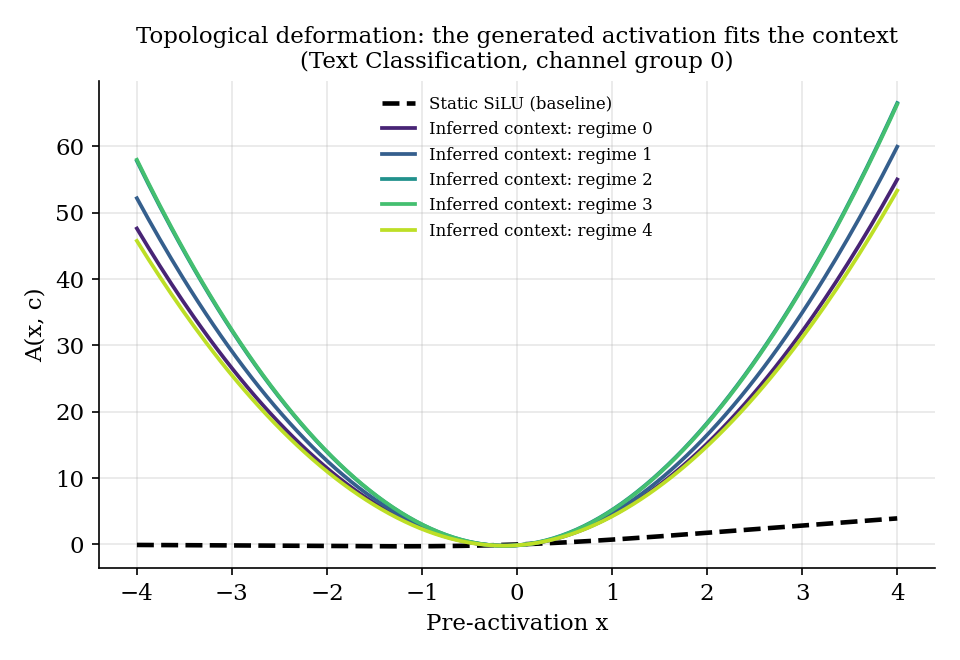
\includegraphics[width=0.47\textwidth]{figs/fig_curves.png}
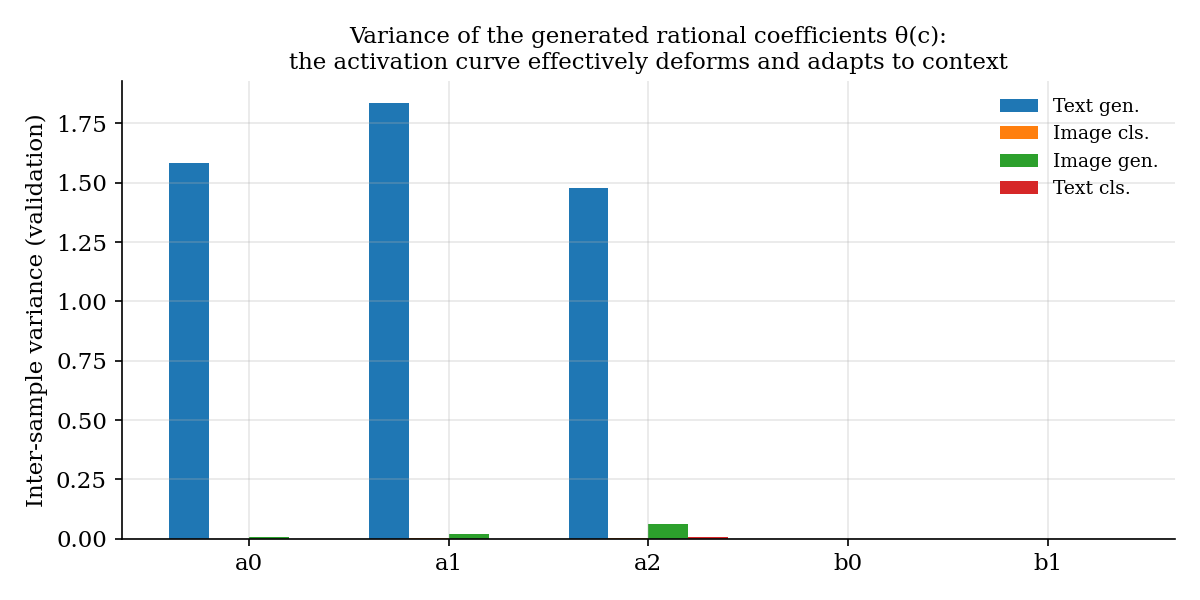
\includegraphics[width=0.47\textwidth]{figs/fig_coeff_var.png}
\caption{Izquierda: curvas generadas para distintos contextos. Derecha: varianza de los coeficientes entre muestras. La adaptación se concentra en el numerador y confirma que el generador no permanece en la inicialización SiLU.}
\label{fig:curves}
\end{figure}

\textbf{Costo.} En texto, CCA-Hinge contiene 82\,276 parámetros y usa 177\,152 FLOPs por muestra. Una iteración compilada de propagación y gradiente tarda 3.823 ms (66\,970 muestras/s). Dynamic ReLU-B requiere 3.656 ms y Meta-ACON 3.681 ms; CCA-Lite requiere 3.747 ms. En dígitos, todos los métodos quedan dentro de $\pm3\%$ de FLOPs; la compilación de Hinge no estuvo disponible en Windows por un error del lanzador Triton, por lo que solo reportamos su medición eager. Las activaciones adaptativas siguen penalizadas por lanzamientos de kernels en redes pequeñas; la proximidad compilada en texto indica que esa latencia es parcialmente fusionable, pero no afirmamos costo real idéntico en todo hardware.

\section{Conclusiones, limitaciones y reproducibilidad}
CCA-Hinge mejora de forma significativa a Dynamic ReLU-B bajo presupuesto igualado en el benchmark real MNIST+SVHN+USPS y obtiene la mejor media en razonamiento, audio y generación corta. En texto queda empatada con los baselines adaptativos, y en sentimiento no mejora a SiLU. La conclusión es específica: condicionar la forma de la activación ayuda cuando el contexto modifica la transformación necesaria; añadir complejidad dinámica a un régimen homogéneo no garantiza beneficio.

El estudio usa backbones pequeños, la generación se limita a tres semillas y 500 pasos en imágenes, y la equivalencia estricta de costo se confirma en dos tareas, mientras la matriz amplia usa el mismo backbone y publica sus diferencias. No evaluamos modelos fundacionales ni cambios de dominio no observados durante entrenamiento. Estas limitaciones impiden extrapolar las ganancias a gran escala.

El código, configuraciones, resultados por semilla, manifiestos SHA-256 y comandos de reproducción se publicarán en el \href{https://github.com/agustinastie2/Context-Conditioned-Rational-Activations}{repositorio público de CCA}.
El entorno registrado usa Python 3.14.4, PyTorch 2.11.0, CUDA 13.0 y una NVIDIA RTX 4070 Laptop. Los datasets no se redistribuyen; las descargas verificables conservan los splits descritos.

\bibliographystyle{splncs04}
\bibliography{referencias}


\end{document}
